%-*- coding: utf-8 -*-
\textcolor[RGB]{46, 116, 181}{\chapter{Initialisation}}
Quelle que soit l’importance des avancées scientifiques et technologiques, c’est le travail des
professionnels de santé qui détermine la qualité et l’efficacité des soins. Dans ce contexte, les soins
nutritionnels, qui portent sur l’évaluation de l’état nutritionnel et l’accompagnement alimentaire des
patients hospitalisés, en interaction étroite avec l’équipe de soin, ne font pas exception. Pour ce
faire, les diététiciens développent des actions de complexité variable, tant au niveau des services de
soins que du système de restauration.

Simultanément, les professionnels doivent faire face à de nouveaux défis, dus aux modifications des
profils épidémiologiques, démographiques et sociaux des populations, ce qui exige la mise en place
de nouvelles compétences et la reconfiguration des stratégies d’action. Pour les diététiciens du
secteur hospitalier, elles ont pour conséquences de nouvelles exigences mentales et surtout
cognitives.

Le niveau de développement industriel de la filière alimentaire française allège la charge de travail
technique des diététiciens, non seulement en ce qui concerne la diversité de matières premières,
mais également dans le domaine du contrôle \enquote{qualité}, tout au long de la chaîne de production. De
la même façon, les nouveaux concepts de production en restauration collective, caractérisés par
l’utilisation de produits pré élaborés et l’innovation technologique des équipements, gagnent
visiblement du terrain dans le secteur hospitalier français.

\section{Définition du problème}
L'élaboration de menus dans un hôpital pour la restauration des patients
est une tâche complexe, et doit tenir compte des différentes pathologies
rencontrées. Faute de moyens (temps et argent) seules quelques grandes
lignes de restauration sont retenues; alors qu'idéalement, chaque
patient devrait pourvoir avoir un repas adapté à sa pathologie.

\section{Vision du projet}
\subsection{Solution envisagée}
Le projet Vitameal a pour objectif de faire correspondre au mieux la planification des régimes et des
prescriptions diététiques aux repas réellement servis au patient. Il consiste en un outil interfaçant la
gestion de production, la prise de commande et le suivi nutritionnel des repas.

\subsection{Périmètre}
C'est un diététicien qui renseigne le profil diététique des patients,
sous les directives des médecins. C'est aussi un diététicien qui élabore
les menus des patients. L'outil élaborera donc
les menus par filtrage des produits correspondants aux profils
diététiques des patients. Pour des raisons de simplifications, nous nous limiterons dans ce projet aux seuls patients adolescents et adultes, à l'exclusion des personnes agées.
\begin{figure}[H]
\label{Modelisation_du _probleme}
  \centering
      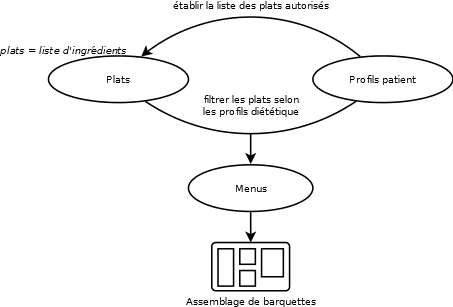
\includegraphics[width=0.75\textwidth]{problem_model} %
\caption{Modélisation du problème}
\end{figure}

\section{Analyse des exigences}
\subsection{Partie prenantes}
\begin{itemize}
\item Participantes~: les diététiciens, le service restauration
\item Concernés~: les médecins, la direction (budget)
\item Impactées~: les patients
\end{itemize}

\subsection{Les besoins}
\begin{description}
\item[] En tant que diététicien, j’ai besoin de :
\begin{description}
 \item[N001:] pouvoir renseigner le profil diététique des patients, afin qu’ils
 puissent bénéficier de menus adaptés.
 \item[N002:] pouvoir élaborer les menus des 3 repas journaliers
 (petit-déjeuner, déjeuner et dîner dont la composition est décrite en annexe
 \ref{annexeA}), de façon automatique, en tenant compte de grammages dépendant du type d'aliments et de la tranche d'age (Document \ref{docNutrition}, Annexe 2).
 \item[N003:] pouvoir saisir des plats et leur composition.
 \item[N004:] élaborer des menus selon les fréquences de service, selon le
 document \ref{docNutrition}, Annexe 4.
 \item[N005:] classer chaque aliment dans une des catégories d’aliments citée
 dans les tables de grammages du document \ref{docNutrition}, Annexes 2 et 4.
\end{description}
\item[N006:] En tant qu’administrateur du site internet de l’hôpital, j’ai
besoin de récupérer le menu de la semaine, afin pouvoir l’intégrer au site.
\item[N007:] En tant que médecin, j’ai besoin de consulter les profils
diététiques des patients admis, pour les  valider.
\item[N008:] En tant que cuisinier du service restauration, j’ai besoin de
consulter les menus élaborés, afin de pouvoir les préparer et prévoir les ingrédients à commander.
\item[N009:] En tant qu’agent de restauration hospitalière,  j’ai besoin de
connaître les menus de chaque patient, afin de pouvoir assembler les plateaux repas.
\end{description}
\subsection{Les contraintes}
\begin{description}
\item[N010:] Les médecins doivent pouvoir vérifier / valider les profils
diététiques des patients.
\item[N011:] La direction fixe un budget maximum par menu.
\end{description}

\subsection{Exigences}

\rowcolors{1}{}{}

\begin{table}[!h]

\begin{tabular}{|p{60mm}p{100mm}|}

\hline

\multicolumn{2}{|l|}{\textbf{REQ\_0100:} 3 repas} \\ \hline

\emph{Type:} Métier & \emph{Liens:} REQ\_0101 REQ\_0105  \\

\emph{Origine:}  & \emph{Validé:} Non \\

\emph{Version:} Initial & \emph{Test:}  \\

\emph{Priorité:} Must & \\ \hline

\multicolumn{2}{|p{16cm}|}{Le système doit permettre de concevoir les 3 repas (petit-déjeuner, déjeuner, souper) d'une journée.} \\ \hline

\end{tabular}

\end{table}



\begin{table}[!h]

\begin{tabular}{|p{60mm}p{100mm}|}

\hline

\multicolumn{2}{|l|}{\textbf{REQ\_0101:} Petit déjeuner} \\ \hline

\emph{Type:} Métier & \emph{Liens:} REQ\_0102 REQ\_0103 REQ\_0104  \\

\emph{Origine:}  & \emph{Validé:} Non \\

\emph{Version:} Initial & \emph{Test:}  \\

\emph{Priorité:} Should & \\ \hline

\multicolumn{2}{|p{16cm}|}{Le système doit permettre de concevoir un petit-déjeuner composé d'une boisson, d'un aliment céréalier, d'un produit laitier et d'un fruit.} \\ \hline

\end{tabular}

\end{table}



\begin{table}[!h]

\begin{tabular}{|p{60mm}p{100mm}|}

\hline

\multicolumn{2}{|l|}{\textbf{REQ\_0102:} Éléments petit déjeuner} \\ \hline

\emph{Type:} Métier & \emph{Liens:}  \\

\emph{Origine:}  & \emph{Validé:} Non \\

\emph{Version:} Initial & \emph{Test:}  \\

\emph{Priorité:} Must & \\ \hline

\multicolumn{2}{|p{16cm}|}{Le système doit permettre de rajouter au petit déjeuner un élément lipidique, sucré ou protodique.} \\ \hline

\end{tabular}

\end{table}



\begin{table}[!h]

\begin{tabular}{|p{60mm}p{100mm}|}

\hline

\multicolumn{2}{|l|}{\textbf{REQ\_0103:} Éléments non diététiques} \\ \hline

\emph{Type:} Métier & \emph{Liens:}  \\

\emph{Origine:}  & \emph{Validé:} Non \\

\emph{Version:} Initial & \emph{Test:}  \\

\emph{Priorité:} Should & \\ \hline

\multicolumn{2}{|p{16cm}|}{Le système doit avertir l'utilisateur de l'usage d'élément non diététique dans un petit déjeuner.} \\ \hline

\end{tabular}

\end{table}



\begin{table}[!h]

\begin{tabular}{|p{60mm}p{100mm}|}

\hline

\multicolumn{2}{|l|}{\textbf{REQ\_0104:} Fréquence éléments non diététiques} \\ \hline

\emph{Type:} Métier & \emph{Liens:}  \\

\emph{Origine:}  & \emph{Validé:} Non \\

\emph{Version:} Initial & \emph{Test:}  \\

\emph{Priorité:} Should & \\ \hline

\multicolumn{2}{|p{16cm}|}{Le système doit vérifier que la fréquence de l'usage d'élément non diététique des petits déjeuners ne dépasse pas 3 repas sur 20, il avertit l'utilisateur si c'est le cas.} \\ \hline

\end{tabular}

\end{table}



\begin{table}[!h]

\begin{tabular}{|p{60mm}p{100mm}|}

\hline

\multicolumn{2}{|l|}{\textbf{REQ\_0105:} Composition déjeuner} \\ \hline

\emph{Type:} Métier & \emph{Liens:}  \\

\emph{Origine:}  & \emph{Validé:} Non \\

\emph{Version:} Initial & \emph{Test:}  \\

\emph{Priorité:} Must & \\ \hline

\multicolumn{2}{|p{16cm}|}{Le système de concevoir un déjeuner et souper composés de 4 ou cinq composantes parmi : entrée, plat protodique, garniture, produit, laitier desserts + de l'eau et du pain (selon le tableau sur la composition du déjeuner en annexe A).} \\ \hline

\end{tabular}

\end{table}



\begin{table}[!h]

\begin{tabular}{|p{60mm}p{100mm}|}

\hline

\multicolumn{2}{|l|}{\textbf{REQ\_0106:} Ajout de plats} \\ \hline

\emph{Type:} Métier & \emph{Liens:}  \\

\emph{Origine:}  & \emph{Validé:} Non \\

\emph{Version:} Initial & \emph{Test:}  \\

\emph{Priorité:} Must & \\ \hline

\multicolumn{2}{|p{16cm}|}{Le système doit permettre d'ajouter des plats et leur définition dans la listes des plats pouvant être préparés.} \\ \hline

\end{tabular}

\end{table}



\begin{table}[!h]

\begin{tabular}{|p{60mm}p{100mm}|}

\hline

\multicolumn{2}{|l|}{\textbf{REQ\_0107:} Description d'un plat} \\ \hline

\emph{Type:} Métier & \emph{Liens:}  \\

\emph{Origine:}  & \emph{Validé:} Non \\

\emph{Version:} Initial & \emph{Test:}  \\

\emph{Priorité:} Must & \\ \hline

\multicolumn{2}{|p{16cm}|}{Le système doit permettre la description d'un plat avec sa liste d'ingrédients et les quantités nécessaires à sa réalisation.} \\ \hline

\end{tabular}

\end{table}



\begin{table}[!h]

\begin{tabular}{|p{60mm}p{100mm}|}

\hline

\multicolumn{2}{|l|}{\textbf{REQ\_0108:} Fréquence de service} \\ \hline

\emph{Type:} Métier & \emph{Liens:}  \\

\emph{Origine:}  & \emph{Validé:} Non \\

\emph{Version:} Initial & \emph{Test:}  \\

\emph{Priorité:} Must & \\ \hline

\multicolumn{2}{|p{16cm}|}{Le système doit proposer un plat selon la fréquence de service de ce plat (exemple 4 fois tous les 20 repas).} \\ \hline

\end{tabular}

\end{table}



\begin{table}[!h]

\begin{tabular}{|p{60mm}p{100mm}|}

\hline

\multicolumn{2}{|l|}{\textbf{REQ\_0410:} Composants des repas} \\ \hline

\emph{Type:} Métier & \emph{Liens:}  \\

\emph{Origine:}  & \emph{Validé:} Non \\

\emph{Version:} Initial & \emph{Test:}  \\

\emph{Priorité:} Must & \\ \hline

\multicolumn{2}{|p{16cm}|}{Le système doit permettre d'ajouter et de supprimer des éléments dans les composants des repas.} \\ \hline

\end{tabular}

\end{table}



\begin{table}[!h]

\begin{tabular}{|p{60mm}p{100mm}|}

\hline

\multicolumn{2}{|l|}{\textbf{REQ\_0411:} Listes par défaut} \\ \hline

\emph{Type:} Métier & \emph{Liens:}  \\

\emph{Origine:}  & \emph{Validé:} Non \\

\emph{Version:} Initial & \emph{Test:}  \\

\emph{Priorité:} Should & \\ \hline

\multicolumn{2}{|p{16cm}|}{Le système doit permettre de revenir aux listes par défaut recommandé par le gouvernement.} \\ \hline

\end{tabular}

\end{table}



\begin{table}[!h]

\begin{tabular}{|p{60mm}p{100mm}|}

\hline

\multicolumn{2}{|l|}{\textbf{REQ\_0500:} Fiche de commande} \\ \hline

\emph{Type:} Métier & \emph{Liens:}  \\

\emph{Origine:}  & \emph{Validé:} Non \\

\emph{Version:} Initial & \emph{Test:}  \\

\emph{Priorité:} Could & \\ \hline

\multicolumn{2}{|p{16cm}|}{Le système doit permettre, une fois les menus élaborés de générer un fiche de commande au format : à définir.} \\ \hline

\end{tabular}

\end{table}



\begin{table}[!h]

\begin{tabular}{|p{60mm}p{100mm}|}

\hline

\multicolumn{2}{|l|}{\textbf{REQ\_0501:} Publication menus} \\ \hline

\emph{Type:} Non Fonctionnelle & \emph{Liens:}  \\

\emph{Origine:}  & \emph{Validé:} Non \\

\emph{Version:} Initial & \emph{Test:}  \\

\emph{Priorité:} Could & \\ \hline

\multicolumn{2}{|p{16cm}|}{Le système doit permettre d'afficher les menus sur un site internet.} \\ \hline

\end{tabular}

\end{table}



\begin{table}[!h]

\begin{tabular}{|p{60mm}p{100mm}|}

\hline

\multicolumn{2}{|l|}{\textbf{REQ\_0600:} Validation des repas} \\ \hline

\emph{Type:} Contrainte & \emph{Liens:}  \\

\emph{Origine:}  & \emph{Validé:} Non \\

\emph{Version:} Initial & \emph{Test:}  \\

\emph{Priorité:} Must & \\ \hline

\multicolumn{2}{|p{16cm}|}{Le système doit gérer un cycle de validation des repas : en cours d'élaboration, en attente de validation, validé.} \\ \hline

\end{tabular}

\end{table}



\begin{table}[!h]

\begin{tabular}{|p{60mm}p{100mm}|}

\hline

\multicolumn{2}{|l|}{\textbf{REQ\_0601:} Droits utilisateurs} \\ \hline

\emph{Type:} Contrainte & \emph{Liens:}  \\

\emph{Origine:}  & \emph{Validé:} Non \\

\emph{Version:} Initial & \emph{Test:}  \\

\emph{Priorité:} Must & \\ \hline

\multicolumn{2}{|p{16cm}|}{Le système doit permettre de gérer différent droit selon le type d'utilisateur.} \\ \hline

\end{tabular}

\end{table}



\begin{table}[!h]

\begin{tabular}{|p{60mm}p{100mm}|}

\hline

\multicolumn{2}{|l|}{\textbf{REQ\_0700:} Menus à assembler} \\ \hline

\emph{Type:} Métier & \emph{Liens:}  \\

\emph{Origine:}  & \emph{Validé:} Non \\

\emph{Version:} Initial & \emph{Test:}  \\

\emph{Priorité:} Must & \\ \hline

\multicolumn{2}{|p{16cm}|}{Le système doit afficher les menu à assembler pour un jour donnée et émettre une étiquette au format : à définir.} \\ \hline

\end{tabular}

\end{table}



\begin{table}[!h]

\begin{tabular}{|p{60mm}p{100mm}|}

\hline

\multicolumn{2}{|l|}{\textbf{REQ\_0701:} Limite prix repas} \\ \hline

\emph{Type:} Contrainte & \emph{Liens:}  \\

\emph{Origine:}  & \emph{Validé:} Non \\

\emph{Version:} Initial & \emph{Test:}  \\

\emph{Priorité:} Must & \\ \hline

\multicolumn{2}{|p{16cm}|}{Le système doit permettre de fixer une limite au prix d'un repas.} \\ \hline

\end{tabular}

\end{table}



\begin{table}[!h]

\begin{tabular}{|p{60mm}p{100mm}|}

\hline

\multicolumn{2}{|l|}{\textbf{REQ\_0702:} Prix repas} \\ \hline

\emph{Type:} Métier & \emph{Liens:}  \\

\emph{Origine:}  & \emph{Validé:} Non \\

\emph{Version:} Initial & \emph{Test:}  \\

\emph{Priorité:} Must & \\ \hline

\multicolumn{2}{|p{16cm}|}{Le système doit permettre de renseigner le prix des éléments d'un repas.} \\ \hline

\end{tabular}

\end{table}



\begin{table}[!h]

\begin{tabular}{|p{60mm}p{100mm}|}

\hline

\multicolumn{2}{|l|}{\textbf{REQ\_0902:} Profil patient} \\ \hline

\emph{Type:} Métier & \emph{Liens:}  \\

\emph{Origine:}  & \emph{Validé:} Non \\

\emph{Version:} Initial & \emph{Test:}  \\

\emph{Priorité:} Must & \\ \hline

\multicolumn{2}{|p{16cm}|}{Le système doit permettre de renseigner un profil patient comportant les éléments suivants : regime particulier(liste à définir), allergie(liste à définir), contre-indication (liste à définir).} \\ \hline

\end{tabular}

\end{table}



\begin{table}[!h]

\begin{tabular}{|p{60mm}p{100mm}|}

\hline

\multicolumn{2}{|l|}{\textbf{REQ\_1000:} État civil} \\ \hline

\emph{Type:} Métier & \emph{Liens:}  \\

\emph{Origine:}  & \emph{Validé:} Non \\

\emph{Version:} Initial & \emph{Test:}  \\

\emph{Priorité:} Must & \\ \hline

\multicolumn{2}{|p{16cm}|}{Le système doit permettre de renseigner l'état civil d'un patient.} \\ \hline

\end{tabular}

\end{table}



\begin{table}[!h]

\begin{tabular}{|p{60mm}p{100mm}|}

\hline

\multicolumn{2}{|l|}{\textbf{REQ\_1001:} Localisation patient} \\ \hline

\emph{Type:} Métier & \emph{Liens:}  \\

\emph{Origine:}  & \emph{Validé:} Non \\

\emph{Version:} Initial & \emph{Test:}  \\

\emph{Priorité:} Must & \\ \hline

\multicolumn{2}{|p{16cm}|}{Le système doit permettre de renseigner la localisation particulière d'un patient.} \\ \hline

\end{tabular}

\end{table}



\begin{table}[!h]

\begin{tabular}{|p{60mm}p{100mm}|}

\hline

\multicolumn{2}{|l|}{\textbf{REQ\_1002:} Grammages} \\ \hline

\emph{Type:} Métier & \emph{Liens:}  \\

\emph{Origine:}  & \emph{Validé:} Non \\

\emph{Version:} Initial & \emph{Test:}  \\

\emph{Priorité:} Must & \\ \hline

\multicolumn{2}{|p{16cm}|}{Le système doit permettre de gérer les grammage de plat.} \\ \hline

\end{tabular}

\end{table}



\begin{table}[!h]

\begin{tabular}{|p{60mm}p{100mm}|}

\hline

\multicolumn{2}{|l|}{\textbf{REQ\_1003:} Plateaux repas} \\ \hline

\emph{Type:} Métier & \emph{Liens:}  \\

\emph{Origine:}  & \emph{Validé:} Non \\

\emph{Version:} Initial & \emph{Test:}  \\

\emph{Priorité:} Must & \\ \hline

\multicolumn{2}{|p{16cm}|}{Le système doit pouvoir gérer des plateaux repas de type : sans régime particulier ou avec régime particulier.} \\ \hline

\end{tabular}

\end{table}



\begin{table}[!h]

\begin{tabular}{|p{60mm}p{100mm}|}

\hline

\multicolumn{2}{|l|}{\textbf{REQ\_1004:} Groupes} \\ \hline

\emph{Type:} Métier & \emph{Liens:}  \\

\emph{Origine:}  & \emph{Validé:} Non \\

\emph{Version:} Initial & \emph{Test:}  \\

\emph{Priorité:} Should & \\ \hline

\multicolumn{2}{|p{16cm}|}{Le système doit gérer les patients par groupes selon leur régime, exemple le groupe des intolérant au lactose.} \\ \hline

\end{tabular}

\end{table}



\begin{table}[!h]

\begin{tabular}{|p{60mm}p{100mm}|}

\hline

\multicolumn{2}{|l|}{\textbf{REQ\_1005:} Génération automatique} \\ \hline

\emph{Type:} Fonctionnelle & \emph{Liens:}  \\

\emph{Origine:}  & \emph{Validé:} Non \\

\emph{Version:} Initial & \emph{Test:}  \\

\emph{Priorité:} Must & \\ \hline

\multicolumn{2}{|p{16cm}|}{Le système doit permettre de générer automatiquement les repas pour un groupe de patients particulier.} \\ \hline

\end{tabular}

\end{table}



\begin{table}[!h]

\begin{tabular}{|p{60mm}p{100mm}|}

\hline

\multicolumn{2}{|l|}{\textbf{REQ\_1006:} Titre} \\ \hline

\emph{Type:} Utilisateur & \emph{Liens:}  \\

\emph{Origine:} Origine & \emph{Validé:} Oui \\

\emph{Version:} Initial & \emph{Test:} Test \\

\emph{Priorité:} Must & \\ \hline

\multicolumn{2}{|p{16cm}|}{le système doit stocker les fiches patients, et permettre de les modifier ou supprimer le cas échéant.} \\ \hline

\end{tabular}

\end{table}



\begin{table}[!h]

\begin{tabular}{|p{60mm}p{100mm}|}

\hline

\multicolumn{2}{|l|}{\textbf{REQ\_1007:} Titre} \\ \hline

\emph{Type:} Utilisateur & \emph{Liens:}  \\

\emph{Origine:} Origine & \emph{Validé:} Oui \\

\emph{Version:} Initial & \emph{Test:} Test \\

\emph{Priorité:} Must & \\ \hline

\multicolumn{2}{|p{16cm}|}{Le système doit permettre de trier les plats par catégories.} \\ \hline

\end{tabular}

\end{table}



\begin{table}[!h]

\begin{tabular}{|p{60mm}p{100mm}|}

\hline

\multicolumn{2}{|l|}{\textbf{REQ\_1008:} Titre} \\ \hline

\emph{Type:} Utilisateur & \emph{Liens:}  \\

\emph{Origine:} Origine & \emph{Validé:} Oui \\

\emph{Version:} Initial & \emph{Test:} Test \\

\emph{Priorité:} Must & \\ \hline

\multicolumn{2}{|p{16cm}|}{Le système doit stocker les intitulés des plats, et permettre leur modification ou leur suppression.} \\ \hline

\end{tabular}

\end{table}





\section{Cas d'utilisations}

\subsection{Cas d'utilisation principal}

\begin{figure}[H]
\centering
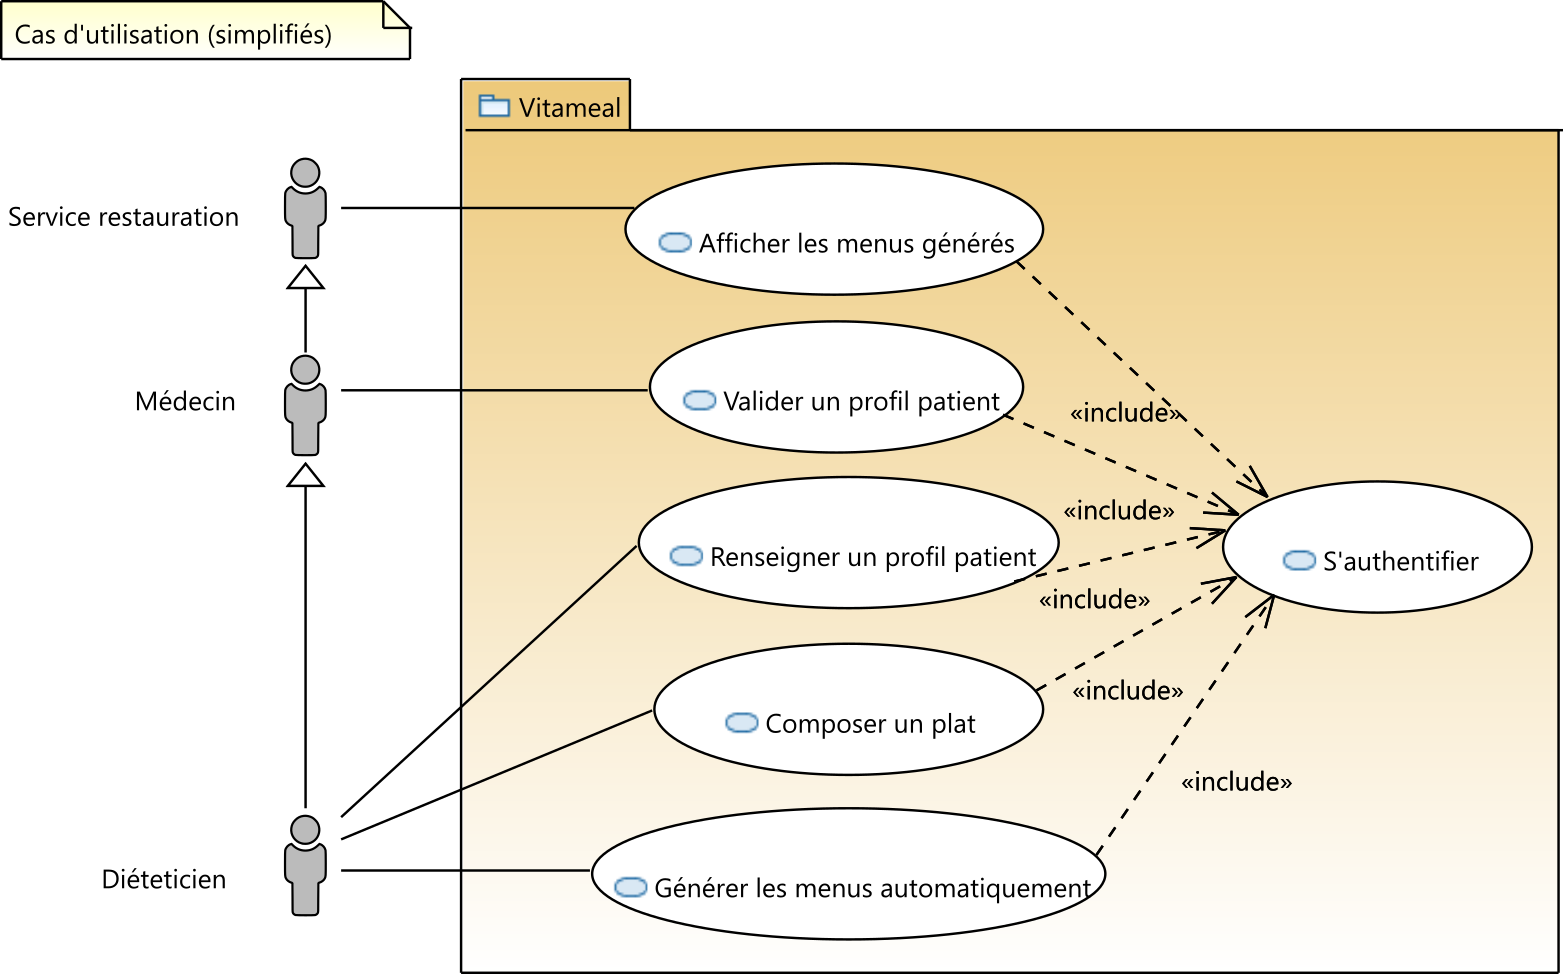
\includegraphics[width=0.9\textwidth]{../../CasDUtilisations/uc_principal.png}
\caption{Cas d'utilisation principal}
\end{figure}

%-*- coding: utf-8 -*-
\subsubsection{Élaboration des menus}
\begin{figure}
  \centering
      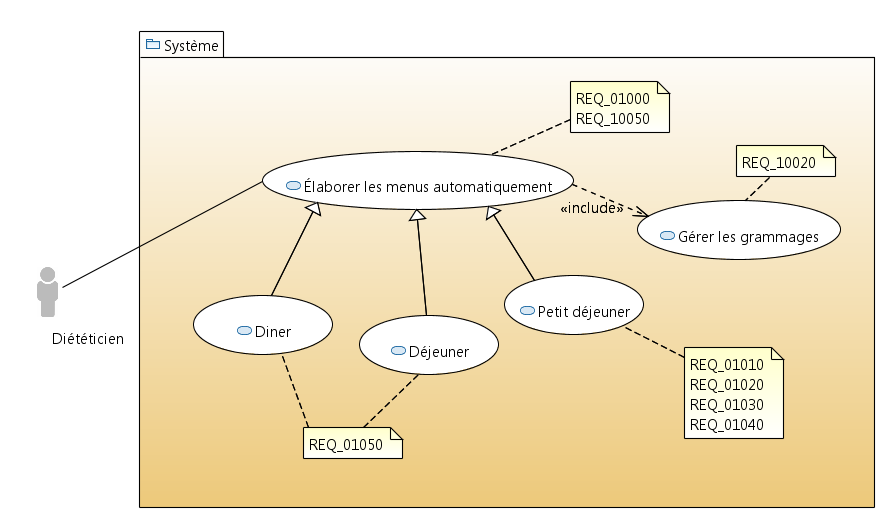
\includegraphics[width=1.00\textwidth]{../../CasDUtilisations/MenuGen/CasDUtilisation/MenuGen.png} %
\caption{Cas d'utilisation élaboration des menus}
\label{MenuGenCU}
\end{figure}

\begin{description}
\item[Nom:] Élaboration des menus (Figure \ref{MenuGenCU}).
\item[ID:] UC300
\item[Description:] Permet l'élaboration des menus.
\item[Auteur:] Jean-Félix BENITEZ.
\item[Date:] 15/06/2017
\item[Acteurs:] Diététiciens.
\item[Pré-Conditions:] Le diététicien s'est connecté au système.
\item[Scénario principal:] Figure \ref{MenuGenSeq}
  \begin{enumerate}
  \item Le diététicien sélectionne le groupe de patients pour lequel il veut générer les menus,
  \item \label{LanceElab}ensuite il lance l'élaboration des menus.
  \item L'élaboration automatique ce déroule en prenant en compte les grammages.
  \item Lorsque les menus sont élaborés, s'il estime l'élaboration correcte, il la valide.
  \item S'il estime l'élaboration incorrecte, il peut la rejeter, auquel cas il reviens à l'étape \ref{LanceElab}
  \item S'il estime l'élaboration incorrecte, il peut aussi la modifier manuellement.
  \end{enumerate}
\item[Scénario alternatif:] Aucun.
\item[Post-Conditions:] Les menus sont générés.
\end{description}

\begin{figure}
  \centering
      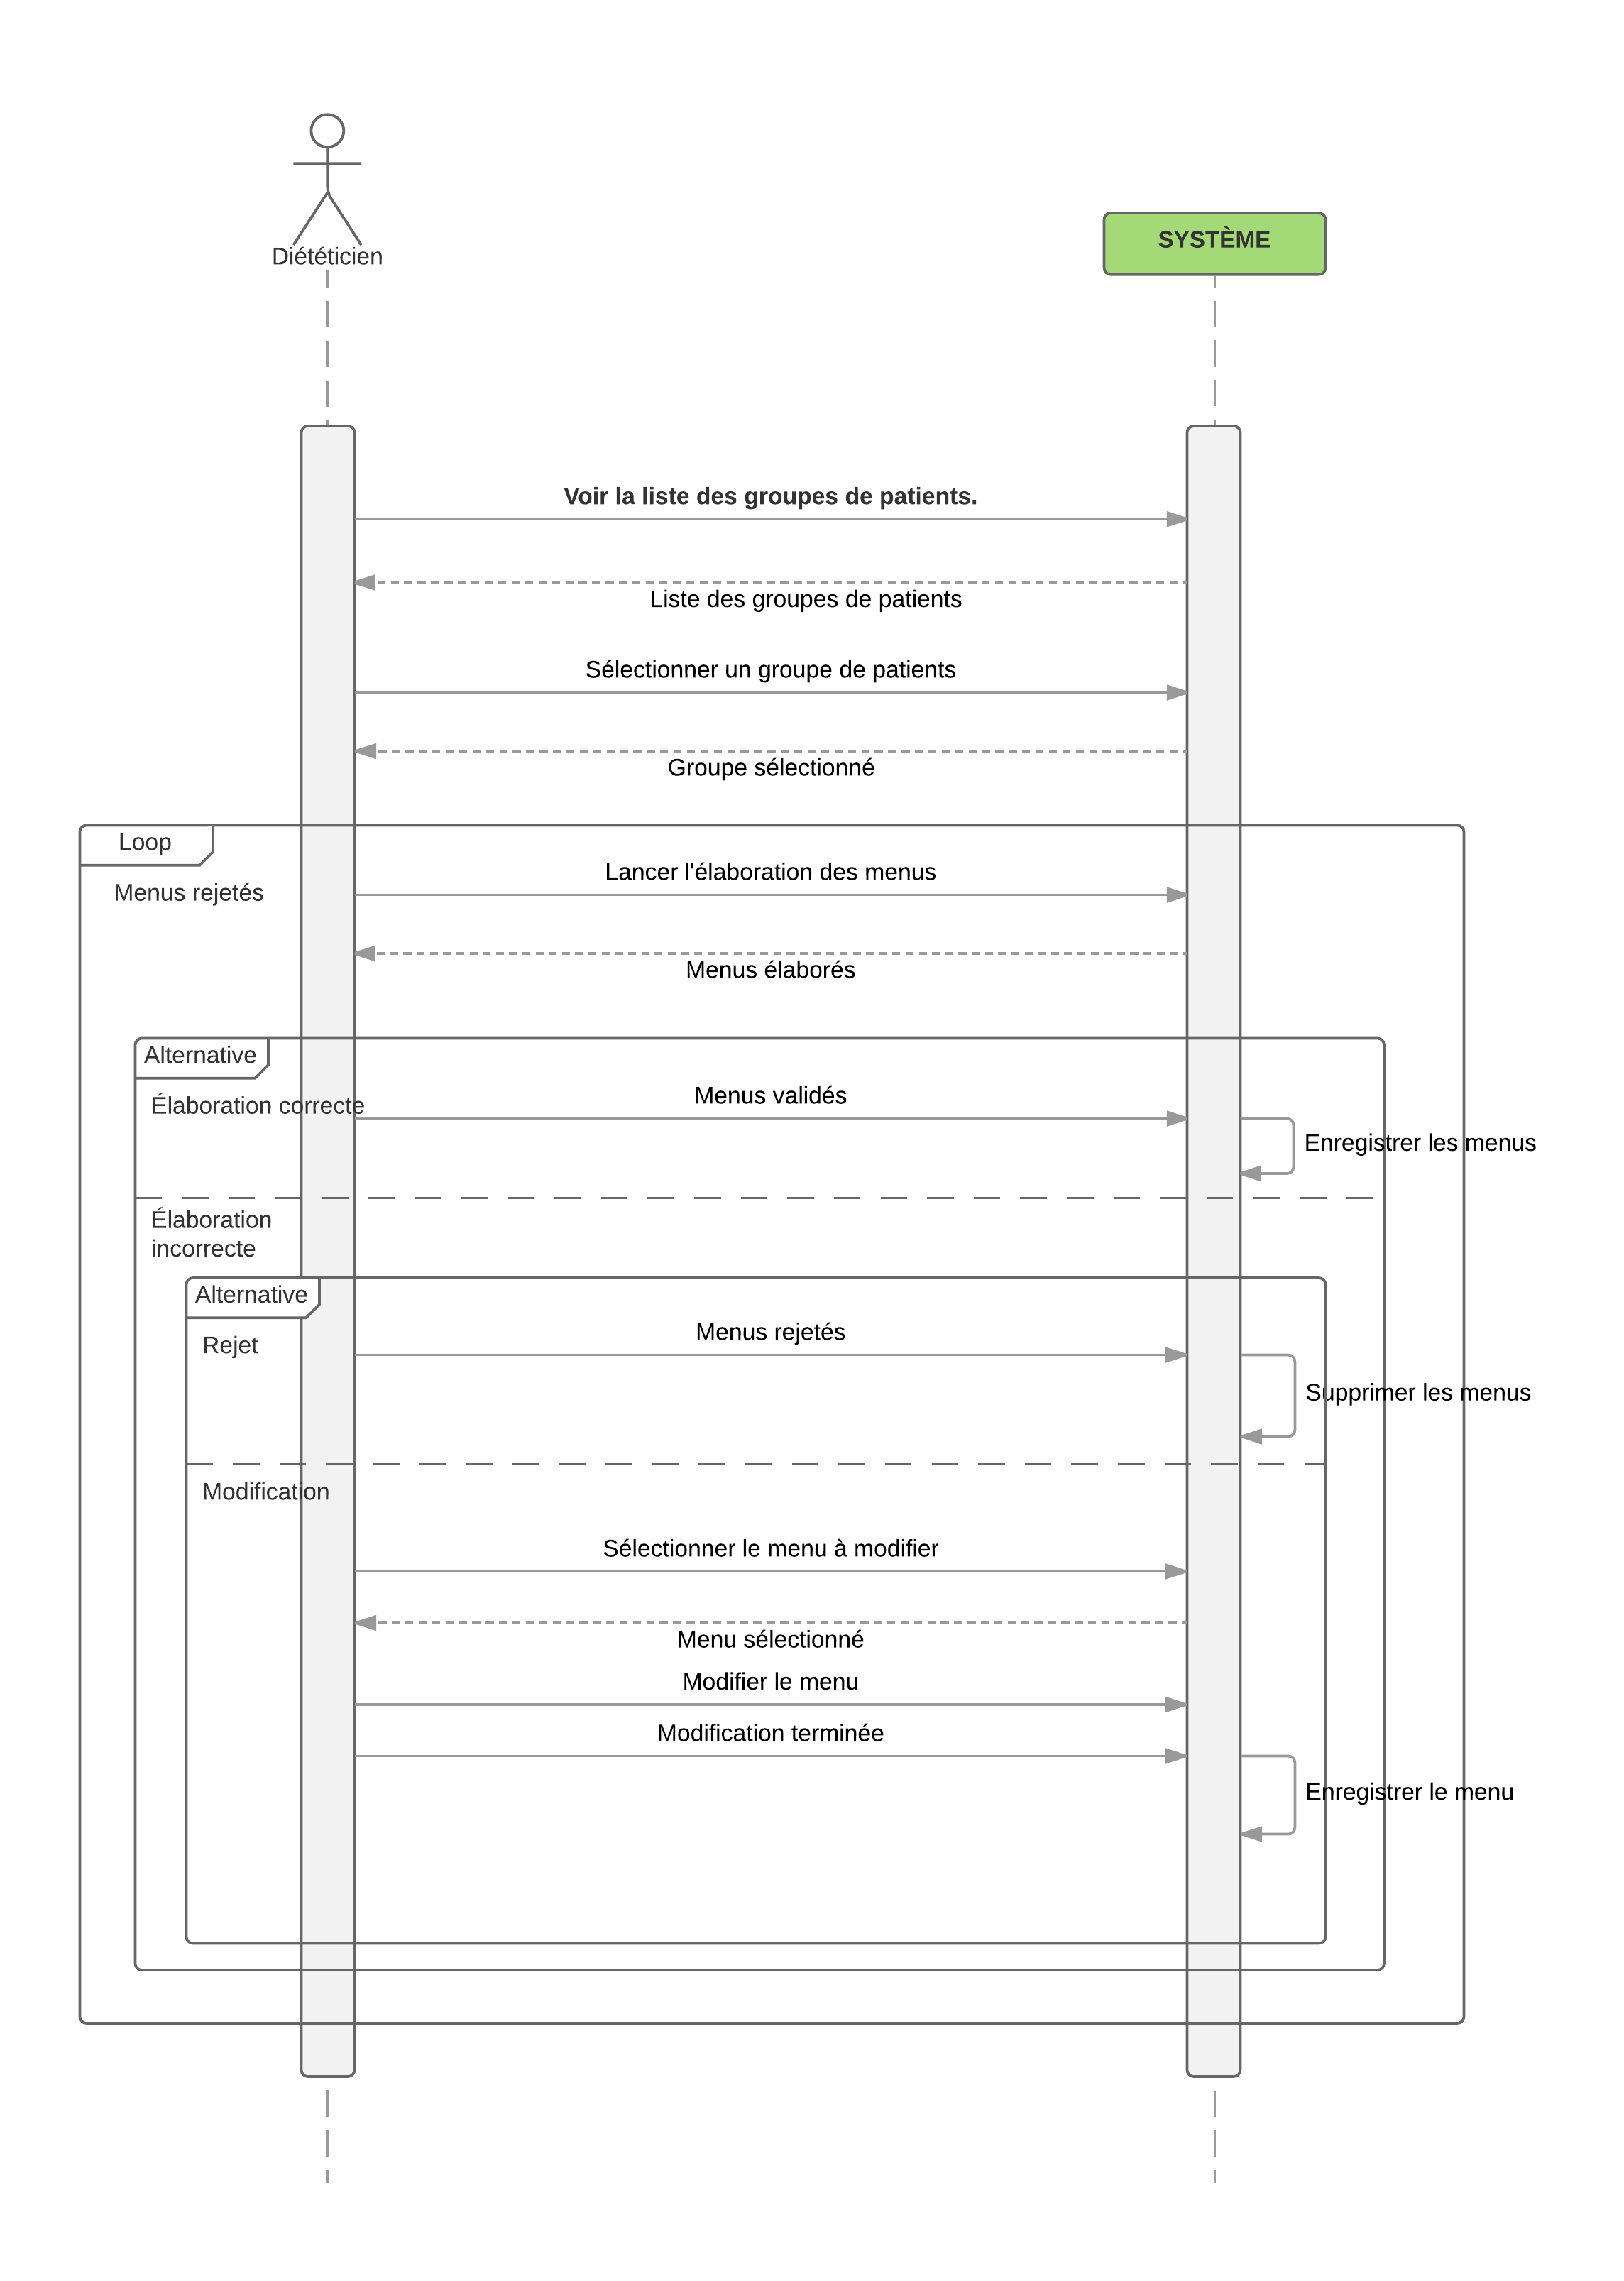
\includegraphics[width=1.00\textwidth]{../../CasDUtilisations/MenuGen/Sequence/ElaborationMenus.png} %
\caption{Séquence élaboration des menus}
\label{MenuGenSeq}
\end{figure}


\subsection{Composer les
plats}\label{diagramme-composer-les-plats}

\begin{figure}
\centering
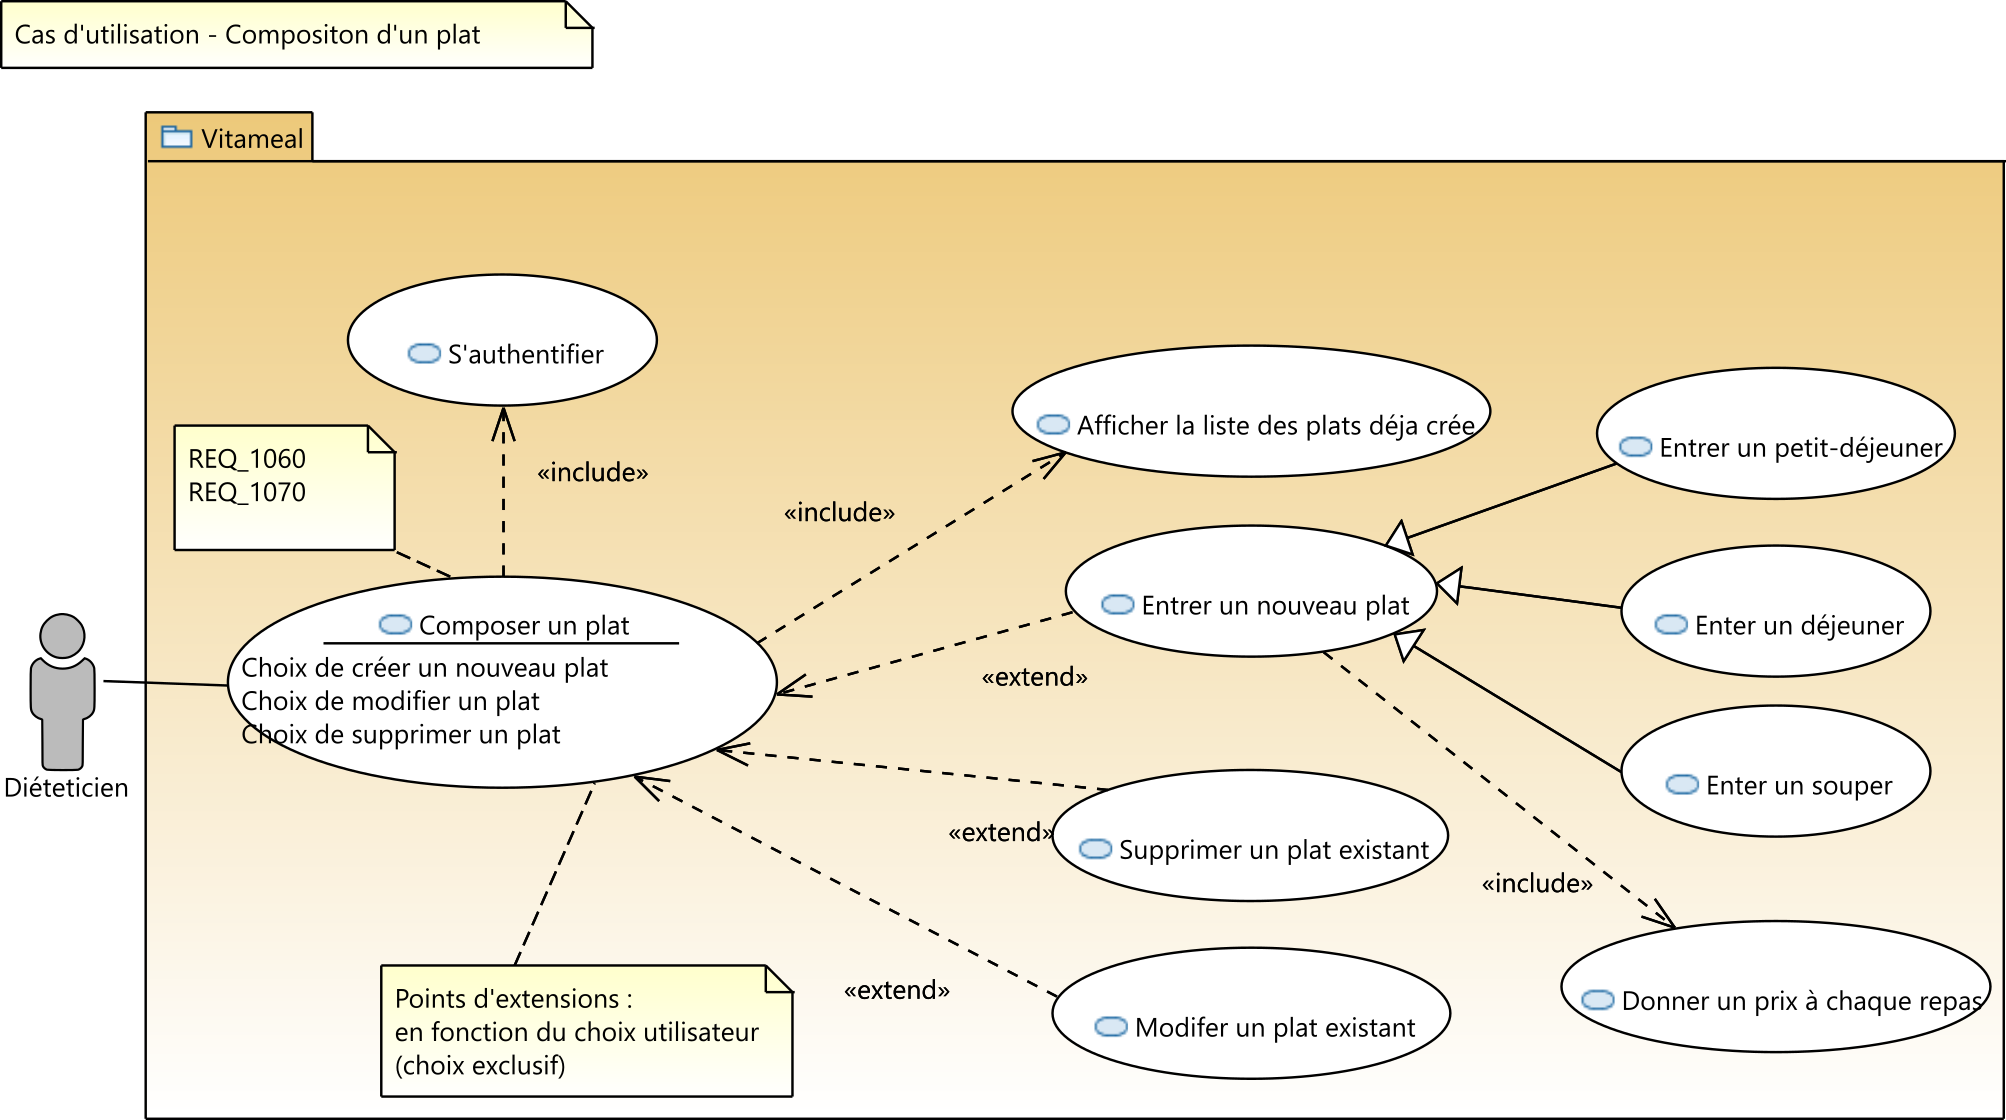
\includegraphics[width=0.9\textwidth]{../../CasDUtilisations/CompositionPlat/uc_composer_un_plat.png}
\caption{Use case composer les plats}
\end{figure}

\subsubsection{UC100 - Composer les
plats}\label{uc100---composer-les-plats}

\noindent\textbf{Nom:} Composer les plats\\
\textbf{ID:} UC100\\
\textbf{Description :} Le diététicien souhaite pouvoir élaborer les
plats composant une journée (petit-déjeuner, déjeuner, souper) en
renseignant leur compositions.\\
\textbf{Auteur :} Nicolas SYMPHORIEN\\
\textbf{Date :} 08/05/2017\\
\textbf{Acteurs :} Le diététicien\\
\textbf{Pré-condition :} L'utilisateur doit être identifié en tant que
diététicien (Voir cas d'utilisation ``S'authentifier'')

\textbf{Scénario principal:}\\
1. Le système affiche la liste des plat déjà créer 2. L'utilisateur
choisi une action :\\
a. L'utilisateur choisi de modifier un plat voir (UC101)\\
b. L'utilisateur choisi de crée un nouveau plat (UC102)\\
c. L'utilisateur choisi de supprimer un plat déjà existant (UC103) 3. Le
système renvoi vers l'écran choisi : ``Modifier un plat'', ``Créer un
plat'' ou affiche une confirmation pour la suppression d'un plat

\textbf{Scénario alternatif:}\\
1. a Le système n'obtient pas la liste des ingrédients

\textbf{Post-Conditions:} L'utilisateur est re-dirigé vers sa sélection.

\subsubsection{UC101 - Modifier un plat
existant}\label{uc101---modifier-un-plat-existant}

\noindent\textbf{Nom:} Modifier un plat existant\\
\textbf{ID:} UC101\\
\textbf{Description :} Le diététicien souhaite pouvoir modifier la
composition d'un plat.\\
\textbf{Auteur :} Nicolas SYMPHORIEN\\
\textbf{Dates :} 08/05/2017\\
\textbf{Acteurs :} Le diététicien\\
\textbf{Pré-condition :} L'utilisateur doit être identifié en tant que
diététicien (Voir cas d'utilisation ``S'authentifier'')

\textbf{Scénario principal :}\\
1. Le système restaure la composition du plat sélectionner et va à
l'étape 3 du cas d'utilisation ``Créer un nouveau plat''

\textbf{Scénario alternatif :}\\
1. a. Le système n'obtient pas la composition du plat sélectionner

\textbf{Post-Conditions:} Le plat est modifié et la modification
enregistrée

\subsubsection{UC102 - Créer un nouveau
plat}\label{uc102---cruxe9er-un-nouveau-plat}

\noindent\textbf{Nom :} Créer un nouveau plat\\
\textbf{ID :} UC102\\
\textbf{Description :} Le diététicien souhaite pouvoir créer la
composition d'un nouveau plat de type petit-déjeuner, déjeuner ou
souper.\\
\textbf{Auteur :} Nicolas SYMPHORIEN\\
\textbf{Dates :} 08/05/2017\\
\textbf{Acteurs :} Le diététicien\\
\textbf{Pré-condition :} L'utilisateur doit être identifié en tant que
diététicien (Voir cas d'utilisation ``S'authentifier'')

\textbf{Scénarios nominal :}\\
1. Le système affiche une page permettant d'entrer la composition d'un
plat 2. L'utilisateur choisi le type de plat (petit-déjeuner, déjeuner,
souper) 3. Le système propose à l'utilisateur une liste de composante à
remplir en fonction du type de plat choisie 4. L'utilisateur choisi les
ingrédients qu'il veut mettre dans chaque composantes 5. L'utilisateur
valide son choix 6. Le système enregistre le nouveau plat dans sa liste
de plats éligible a la composition des menus

\textbf{Scénarios alternatif :}

\begin{enumerate}
\def\labelenumi{\arabic{enumi}.}
\setcounter{enumi}{2}
\item
  \begin{enumerate}
  \def\labelenumii{\alph{enumii}.}
  \item
    L'utilisateur change de type de plat en cours d'élaboration\\
  \end{enumerate}
\item
  \begin{enumerate}
  \def\labelenumii{\alph{enumii}.}
  \setcounter{enumii}{1}
  \item
    Le système propose à l'utilisateur la liste de composante
    correspondante à son nouveau choix (retour etape 3.)\\
  \end{enumerate}
\item
  \begin{enumerate}
  \def\labelenumii{\alph{enumii}.}
  \setcounter{enumii}{2}
  \item
    Le système n'obtient pas la composition du liste des ingrédients\\
  \end{enumerate}
\item
  \begin{enumerate}
  \def\labelenumii{\alph{enumii}.}
  \item
    L'utilisateur annule la composition du plat
  \end{enumerate}
\end{enumerate}

\textbf{Post-Conditions:} Le plat est crée et enregistré

\subsubsection{UC103 - Supprimer un
plat}\label{uc103---supprimer-un-plat}

\noindent\textbf{Nom :} Supprimer un plat\\
\textbf{ID :} UC103\\
\textbf{Description :} Le diététicien souhaite pouvoir supprimer un
plat.\\
\textbf{Auteur :} Nicolas SYMPHORIEN\\
\textbf{Dates :} 08/05/2017\\
\textbf{Acteurs concernés :} Le diététicien\\
\textbf{Pré-condition :} L'utilisateur doit être identifié en tant que
diététicien (Voir cas d'utilisation ``S'autentifier'')

\textbf{Scénarios nominal :}

\begin{enumerate}
\def\labelenumi{\arabic{enumi}.}
\item
  Le système affiche un message d'avertissement avant la suppression
\item
  L'utilisateur confirme ou non la suppression
\item
  Le système supprime le plat de sa liste des plats
\end{enumerate}

\textbf{Scénarios alternatif :}

\begin{enumerate}
\def\labelenumi{\arabic{enumi}.}
\setcounter{enumi}{2}
\item
  \begin{enumerate}
  \def\labelenumii{\alph{enumii}.}
  \item
    Le système ne réussi pas à supprimer le plat
  \end{enumerate}
\end{enumerate}

\textbf{Post-Conditions:} Le plat est supprimé

\subsubsection{UC202 - Donner un prix à chaque
repas}\label{uc202---donner-un-prix-uxe0-chaque-repas}

\noindent\textbf{Nom :} Donner un prix à chaque repas\\
\textbf{ID :} UC202\\
\textbf{Description :} Le service restauration souhaite pouvoir donnée
le pris de chaque plat composant un menu\\
\textbf{Auteur :} Nicolas SYMPHORIEN\\
\textbf{Dates(s) :} 08/05/2017\\
\textbf{Acteurs :} Le service restauration, par héritage, le diététicien
et le médecin\\
\textbf{Pré-condition :} L'utilisateur doit être identifié

\textbf{Scénario principal :}\\
1. Le système propose de renseigner le prix du plat

\textbf{Scénario alternatif :} aucun

\textbf{Post-Conditions:} Le prix du plat est renseigné


\subsection{Diagramme afficher les menus
générés}\label{diagramme-afficher-les-menus-guxe9nuxe9ruxe9s}

\begin{figure}
\centering
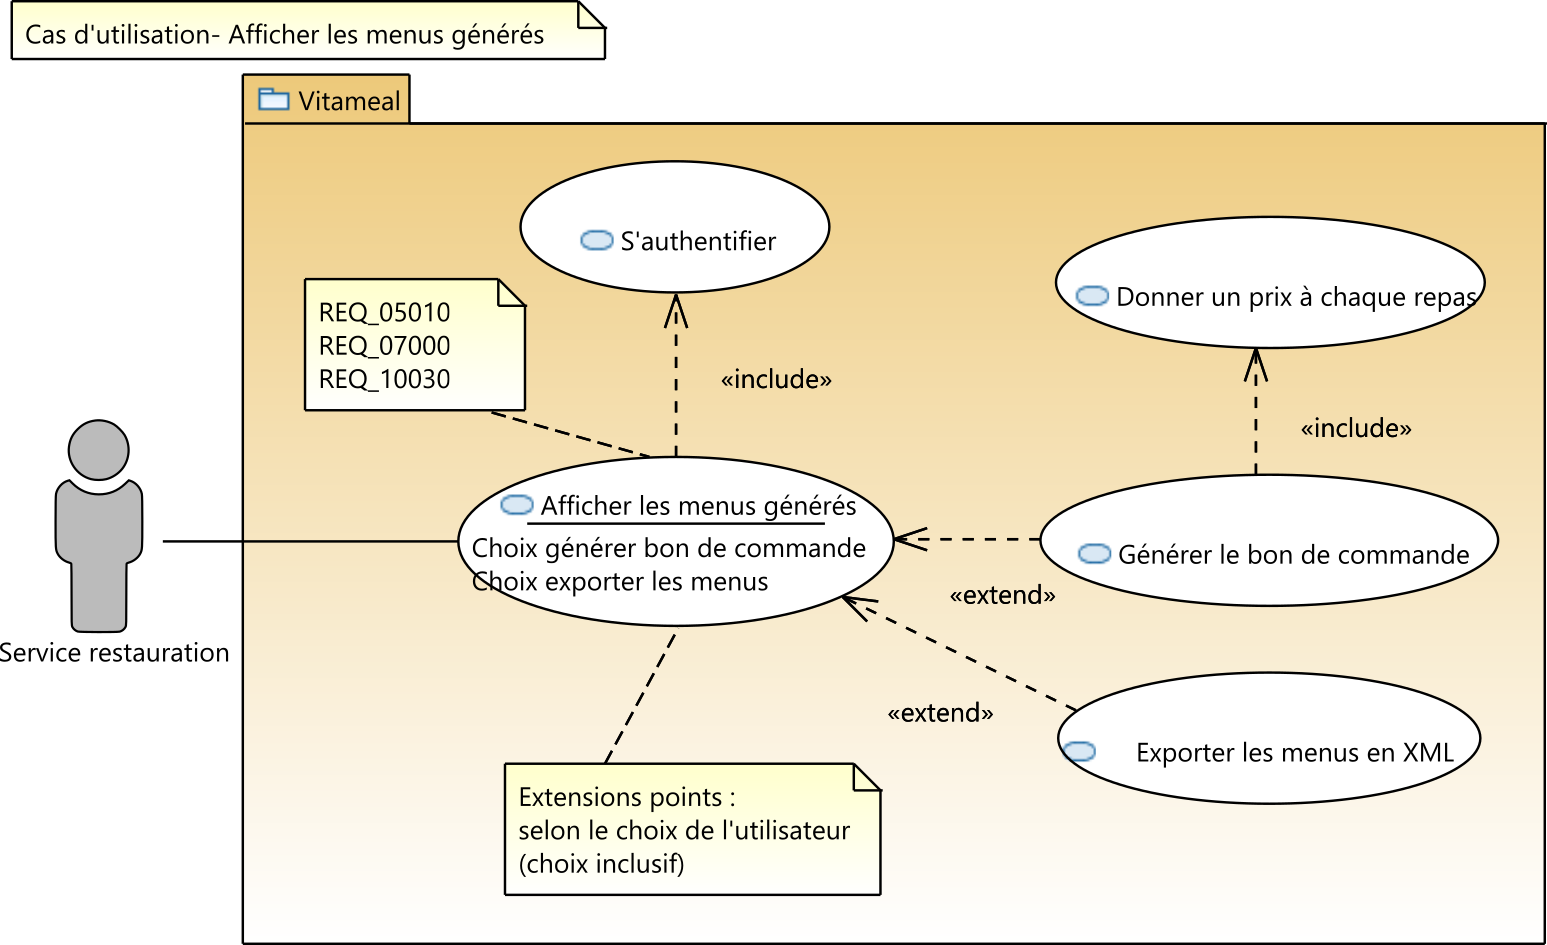
\includegraphics[width=0.85\textwidth]{../../CasDUtilisations/AfficherMenu/uc_afficher_menu.png}
\caption{Use case afficher les menus générés}
\end{figure}

\subsubsection{UC200 - Afficher les menus
générés}\label{uc200---afficher-les-menus-guxe9nuxe9ruxe9s}

\noindent\textbf{Nom :} Modifier un plat existant\\
\textbf{ID :} UC200\\
\textbf{Description :} Le service restauration souhaite pouvoir voir le
menu généré et selon son choix imprimer un bon\\
de commande et/ou exporter le menu sous un autre format.\\
\textbf{Auteur :} Nicolas SYMPHORIEN\\
\textbf{Dates(s) :} 08/05/2017\\
\textbf{Acteurs :} Le service restauration, par héritage, le diététicien
et le médecin\\
\textbf{Pré-condition :} L'utilisateur doit être identifié

\textbf{Scénario principal :}\\
1. Le système affiche un menu pour un groupe de patient donné 2.
L'utilisateur peut choisir de générer et voir le bon de commande associé
au menu affiché et l'utilisateur peut choisir de exporter le menu (pour
un usage par une tierce application)

\textbf{Scénario alternatif :}\\
1.a L'utilisateur peut changer de groupe de patient 1.b Le système
n'arrive pas à récupérer les menu générés 1.c Le système ne possède pas
de menu généré, il affiche un message d'information à l'utilisateur

\textbf{Post-Conditions:} Le menu est affiché. Un bon de commande est
produit. Un export est produit.

\subsubsection{UC201 - Générér le bon de
commande}\label{uc201---guxe9nuxe9ruxe9r-le-bon-de-commande}

\noindent\textbf{Nom :} Générer le bon de commande\\
\textbf{ID :} UC201\\
\textbf{Description :} Le service restauration souhaite pouvoir imprimer
un bon de commande du menu affiché\\
\textbf{Auteur :} Nicolas SYMPHORIEN\\
\textbf{Dates(s) :} 08/05/2017\\
\textbf{Acteurs :} Le service restauration, par héritage, le diététicien
et le médecin\\
\textbf{Pré-condition :} L'utilisateur doit être identifié

\textbf{Scénario principal :}\\
1. Le système propose la génération du menu si le prix de chaque plat a
été renseigné

\textbf{Scénario alternatif :}\\
1. a. Le prix de chaque plat n'a pas été renseigné

\textbf{Post-Conditions:} Le bon de commande et généré et affiché.

\subsubsection{UC202 - Donner un prix à chaque
repas}\label{uc202---donner-un-prix-uxe0-chaque-repas}

\noindent\textbf{Nom :} Donner un prix à chaque repas\\
\textbf{ID :} UC202\\
\textbf{Description :} Le service restauration souhaite pouvoir donnée
le pris de chaque plat composant un menu\\
\textbf{Auteur :} Nicolas SYMPHORIEN\\
\textbf{Dates(s) :} 08/05/2017\\
\textbf{Acteurs :} Le service restauration, par héritage, le diététicien
et le médecin\\
\textbf{Pré-condition :} L'utilisateur doit être identifié

\textbf{Scénario principal :}\\
1. Le système propose de renseigner le prix du plat

\textbf{Scénario alternatif :} aucun

\textbf{Post-Conditions:} Le prix du plat est renseigné

\subsubsection{UC203 - Exporter le menu affiché au format
XML}\label{uc203---exporter-le-menu-affichuxe9-au-format-xml}

\noindent\textbf{Nom :} Exporter le menu affiché au format XML\\
\textbf{ID :} UC203\\
\textbf{Description :} Le service restauration souhaite pouvoir exporté
le menu affiché pour un usage dans une tierce application (comme le site
internet de l'hopital par exemple)\\
\textbf{Auteur :} Nicolas SYMPHORIEN\\
\textbf{Dates(s) :} 08/05/2017\\
\textbf{Acteurs :} Le service restauration, par héritage, le diététicien
et le médecin\\
\textbf{Pré-condition :} L'utilisateur doit être identifié

\textbf{Scénario principal :}\\
1. Le système exporte le menu affiché en XML

\textbf{Scénario alternatif :} échec de l'export

\textbf{Post-Conditions:} Le menu est exportée au format XML


%-*- coding: utf-8 -*-
\section{Backlog}
\subsection{Profil patient}
\begin{enumerate}
\item En tant que diététicien, je souhaite pouvoir créer un profil patient.
\item En tant que diététicien, je souhaite pouvoir renseigner un profil patient comportant les éléments suivants : nom, prénom, date de naissance.
\item En tant que diététicien, je souhaite pouvoir renseigner des allergies éventuelles dans le profil patient.
\item En tant que diététicien, je souhaite pouvoir renseigner un régime alimentaire prescrit, en choisissant entre les items suivants : régime sans sel, régime sans sucre, régime sans matières grasses, régime sans gluten, régime sans lactose.
\item En tant que diététicien, je souhaite pouvoir modifier un profil patient.
\item En tant que diététicien, je souhaite pouvoir supprimer un profil patient.
\item En tant que diététicien, je souhaite pouvoir gérer les patients par groupes selon leur régime prescrit, exemple le groupe des intolérants au lactose.
\item En tant que médecin, je souhaite pouvoir valider le profil diététique du patient, en plus d'effectuer toutes les actions réalisables par le diététicien.
\end{enumerate}

\subsection{Composition des plats}
\begin{enumerate}
\item En tant que diététicien, je souhaite pouvoir ajouter des plats et leurs définitions dans la listes des plats pouvant être préparés.
\item En tant que diététicien, je souhaite pouvoir descrire un plat avec sa liste d'ingrédients et les quantités nécessaires à sa réalisation.
\item Le système doit proposer un plat selon la fréquence de service de ce plat (exemple 4 fois tous les 20 repas).
  \end{enumerate}

